\documentclass[border=4pt]{standalone}
\usepackage{amsmath,amssymb,tikz}\usetikzlibrary{arrows.meta}
\definecolor{figB}{RGB}{31,90,166}\definecolor{figR}{RGB}{176,48,48}\definecolor{figG}{RGB}{46,125,50}\definecolor{figO}{RGB}{214,120,20}
% Left: (2 1; 1 2), eigenvalues 3 on (1,1), 1 on (1,-1). Right: (2 1; 0 3), eigenvalues 2 on (1,0), 3 on (1,1).
\begin{document}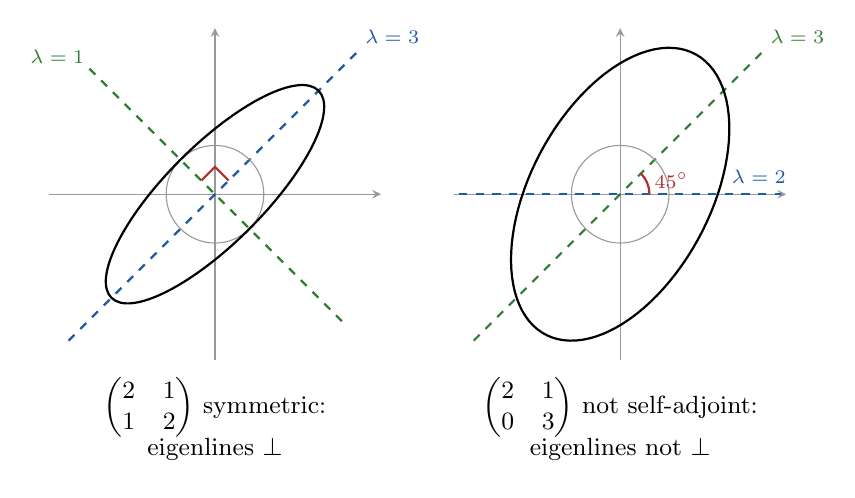
\begin{tikzpicture}[scale=0.62,>={Stealth[length=1.8mm]}]
\begin{scope}
\draw[black!40,thin,-stealth] (-3.4,0)--(3.4,0); \draw[black!40,thin,-stealth] (0,-3.4)--(0,3.4);
\draw[dashed,thick,figB] (-3,-3)--(3,3) node[above right,font=\scriptsize,inner sep=1pt]{$\lambda=3$};
\draw[dashed,thick,figG] (2.6,-2.6)--(-2.6,2.6) node[above left,font=\scriptsize,inner sep=1pt]{$\lambda=1$};
\draw[black!40] (0,0) circle (1); \draw[thick,rotate=45] (0,0) ellipse (3 and 1);
\draw[thick,figR] (0.28,0.28)--(0,0.56)--(-0.28,0.28);
\node[font=\small,align=center] at (0,-4.6) {$\begin{pmatrix}2&1\\1&2\end{pmatrix}$ symmetric:\\[-1pt] eigenlines $\perp$};
\end{scope}
\begin{scope}[xshift=8.3cm]
\draw[black!40,thin,-stealth] (-3.4,0)--(3.4,0); \draw[black!40,thin,-stealth] (0,-3.4)--(0,3.4);
\draw[dashed,thick,figB] (-3.3,0)--(3.3,0) node[above,font=\scriptsize,pos=0.93]{$\lambda=2$};
\draw[dashed,thick,figG] (-3,-3)--(3,3) node[above right,font=\scriptsize,inner sep=1pt]{$\lambda=3$};
\draw[black!40] (0,0) circle (1);
\draw[thick,domain=0:360,samples=100] plot ({2*cos(\x)+sin(\x)},{3*sin(\x)});
\draw[thick,figR] (0.6,0) arc (0:45:0.6); \node[font=\scriptsize,figR] at (1.05,0.28) {$45^\circ$};
\node[font=\small,align=center] at (0,-4.6) {$\begin{pmatrix}2&1\\0&3\end{pmatrix}$ not self-adjoint:\\[-1pt] eigenlines not $\perp$};
\end{scope}
\end{tikzpicture}\end{document}
